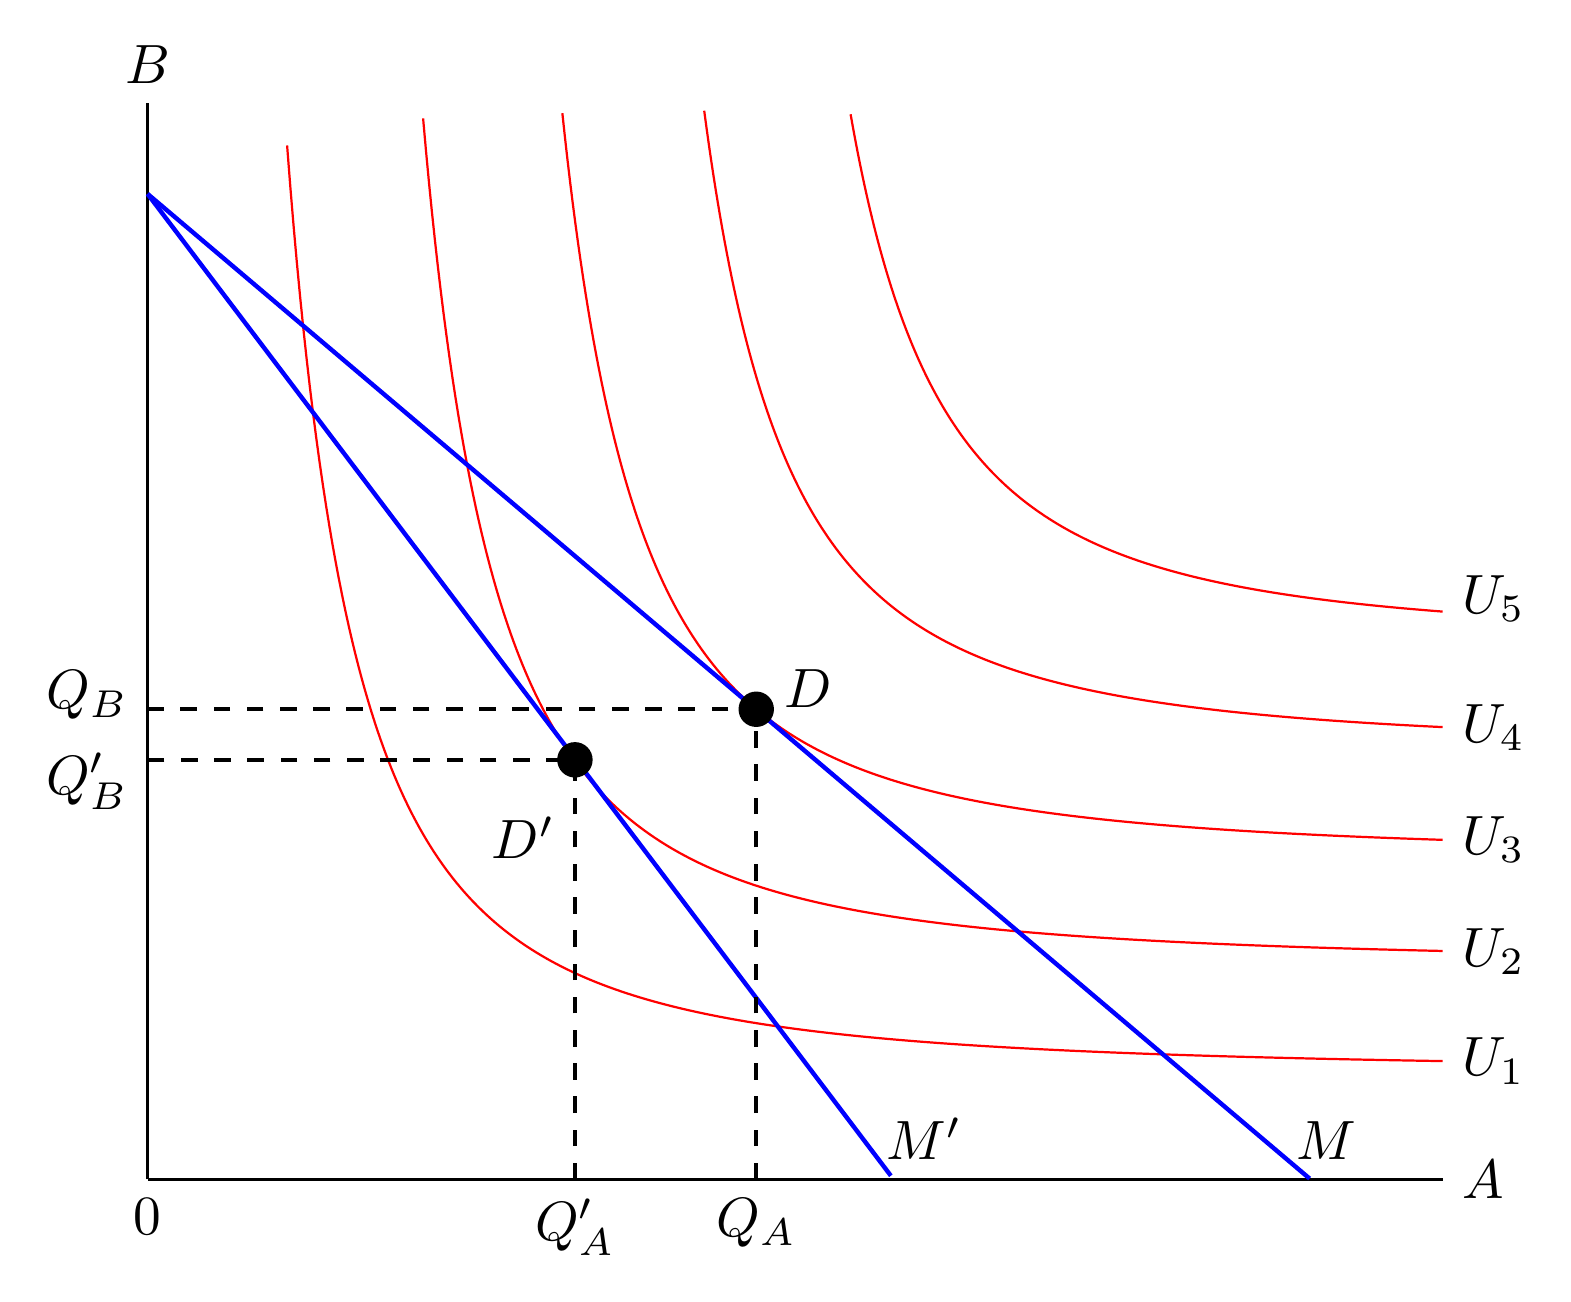
\begin{tikzpicture}[scale=2]
\begin{axis}[
scale = 1.2,
xmin = 0, xmax = 10,
ymin = 0, ymax = 10,
axis lines* = left,
xtick = {0}, ytick = \empty,
clip = false,
]
% Indifference curves
\addplot[domain = 0:10, restrict y to domain = 0:10, samples =
   400, color = red]{10/(x^2)+1};
\addplot[domain = 1:10, restrict y to domain = 0:10, samples =
   400, color = red]{10/((x-1)^2)+2};
\addplot[domain = 2:10, restrict y to domain = 0:10, samples =
   400, color = red]{10/((x-2)^2)+3};
\addplot[domain = 3:10, restrict y to domain = 0:10, samples =
   400, color = red]{10/((x-3)^2)+4};
\addplot[domain = 4:10, restrict y to domain = 0:10, samples =
   400, color = red]{10/((x-4)^2)+5};
% Budget constraints
\addplot[domain = 0:10, restrict y to domain = 0:10, samples =
   400, color = blue, thick]{9.16-1.02*x};
\addplot[domain = 0:10, restrict y to domain = 0:10, samples =
   400, color = blue, thick]{9.16-1.59*x};
% Dashed lines
\addplot[color = black, dashed, thick] coordinates {(4.7, 0) (4.7,
    4.37) (0, 4.37)};
\addplot[color = black, dashed, thick] coordinates {(3.3, 0) (3.3,
    3.9) (0, 3.9)};
% Coordinate points
\addplot[color = black, mark = *, only marks, mark size = 3pt]
   coordinates {(3.3, 3.9) (4.7, 4.37)};
% Labels
\node [right] at (rel axis cs:1,0) {$A$};
\node [above] at (rel axis cs:0,1) {$B$};
\node [above] at (9.1, 0) {$M$};
\node [above] at (6, 0) {$M^\prime$};
\node [below] at (4.7, 0) {$Q_A$};
\node [below] at (3.3, 0) {$Q_A^\prime$};
\node [left] at (0, 4.5) {$Q_B$};
\node [left] at (0, 3.7) {$Q_B^\prime$};
\node [above] at (5.1, 4.2) {$D$};
\node [above] at (2.9, 2.8) {$D^\prime$};
\node [right] at (10, 1.1) {$U_1$};
\node [right] at (10, 2.12) {$U_2$};
\node [right] at (10, 3.16) {$U_3$};
\node [right] at (10, 4.2) {$U_4$};
\node [right] at (10, 5.4) {$U_5$};
\end{axis}
\end{tikzpicture}